\chapter{Method}

Our approach was to formulate a basic plan of attack that was feasible to accomplish in a timespan of three months.
%
The main tasks were:
\begin{itemize}
\item Outline the concept and interaction of components.
\item Design sensor prototype software.
\item Design sink and authentication server software.
\item Implementation of the necessary cryptographic primitives.
\item Design and implementation of cryptographic protocols for authentication, re-keying and data transfer.
\item Integration and testing of a test-bed system.
\end{itemize}


\subsection{The TSense system}

The TSense system is shown in its simplest form in Figure~\ref{fig:sys-overview}. The module types are

\begin{description}
\item \textbf{Trusted sensor -- tsensor -- ($T$)} measures some array of quantities, e.g.\ temperature, pollutant particle count or luminosity, and publishes in an authenticated manner to a client ($C$). The published results may additionally be encrypted. tsensor would be tamper-proof in a production setting.
\item \textbf{Client ($C$)} hosts the sensor, e.g.\ physically attached or USB-connected. The client is the corruptible (adversary controlled) entity in our model, as further discussed in Section~\ref{}. A honest client will always forward measurements unmodified to the sink $S$, whereas a corrupted $C$ may attempt modify the readings. We simplify our present model so that each $C$ hosts exactly one sensor $T$. Further, each $C$ communicates directly with exactly one sink server $S$.
\item \textbf{Sink server ($S$)} collects measurements forwarded from a number of $C$ nodes. A network may include multiple networked sinks to achieve some degree of scalability. In such a system, each of the sinks is a \textit{clusterhead} for a number of clients. In this work, we regard all $S$ to be trusted. This is a simplifying assumption that will be relaxed in future work.
\item \textbf{Authentication service ($A$)} handles authentication of sensor nodes and clients at time of insertion into a working measurement network. Even though we regard the $S$ to be trusted, it is a prudent measure to limit the distribution of sensor private keys. In our model, we limit the distribution of the private sensor keys to $T$ and $A$ nodes. We regard $A$ to be incorruptible (unconditionally). A single $A$ is assumed, which is a somewhat reasonable assumption from a scalability standpoint, since authentication takes place much less frequently than data collection.
%We assume the authentication service $A$ is accessed only by $s \in S$, and never directly by any $c \in C$. This simply limits the exposure potential of $A$ to adversaries. In this project, we implicitly assume perfect mutual trust between any $s$ and $A$. In reality, measures would have to be taken to harden $A$, but this task is eased by limiting the population of nodes which have access to it. All communications between $A$ and $s_j$ are encrypted, as a TLS/SSL tunnel and mutual authentication assumed. Additionally, we can use asymmetric crypto to add a further layer of security to the exchange.
\end{description}

\begin{figure}
\begin{center}
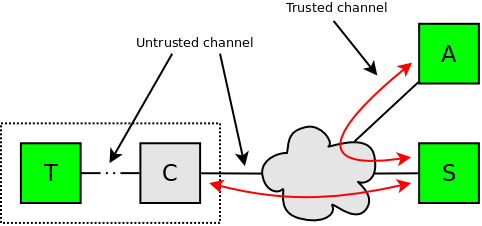
\includegraphics[width=0.6\textwidth]{figures/sys-overview.png} 
\end{center}
\caption{System overview. Interaction of the entities of the system. Green: Trusted entities. Gray: Untrusted entities (compromizable), Black channels: Insecure, Red channels: Secure.}
\label{fig:sys-overview}
\end{figure}

%All channels are regarded as untrusted. However, protection against outsider adversaries is assumed to be prevented by standard cryptographic primitives -- shared key encryption between sensor and sink and TLS with mutual authentication between sink and authentication servers.

The tsensor and tsclient communicate over a serial link, provided by an USB-serial emulator. The tsclient, and by extension both of its communications channels, are considered untrusted. The tsensor and tsclient communicate using a dedicated communications protocol (partly secured by the tsensor), further described in Section~\ref{}. However, tsclient plays no part in the system security.

tsclient and tsink communicate over an IP network, using TCP/IP and a set of dedicated protocols described in Section~\ref{}. Other transport layer protocols than TCP may indeed be used; our decision to use standard socket communications was merely one of convenience. Indeed, we may consider unreliable wireless communications protocols in our future work. tsclient and tsink use a standard unencrypted TCP connection; all security is provided by tsensor/tsink operations, rendering critical operations inaccessible and unmodifiable (within computational bounds) by the untrusted tsclient or any third parties.

tsink and tauth communicate over an IP network, using TLS \cite{} and TCP-IP. TLS provides strong mutual authentication, confidentiality and integrity for message transfer between these two critical system types. A bit of security-by-obscurity can be assumed by using non-standard ports.  

\subsection{System design decisions}

The main design decisions for the system were formulated and decided upon early on.

\begin{enumerate}
\item We wanted the system to be as simple as possible while at the same time giving reasonable guarantees of authenticity.
\item We wanted the sensor to be compact and cheap as possible, almost a disposable unit. The closest practical alternative was to use an Arduino prototyping board. The sensor hardware and software is further described in Section~\ref{}.
\item We wanted the cryptographic primitives used for encryption and tagging to be as strong as possible, considering the severely resource constrained sensor hardware. The resource constraints prompted us to use strictly symmetric (shared key), rather than asymmetric (public key) cryptography. At the same time, we wanted to use publicly available algorithms. We considered the very compact XTEA \cite{} algorithm initially, but decided upon the industry standard AES \cite{} block cipher. The implementation of the cryptographic primitives is described in Section~\ref{}.
\item We wanted the algorithms to be as efficient as possible to reduce resource use (memory, CPU, networking) on all system components.
\item We wanted the overall system to be as simple as possible -- that is, we wanted to determine the minimum support a trusted sensor needs to achieve our required level of security.
\end{enumerate}
\textbf{IS THIS PERHAPS A MIX OF REQUIREMENTS AND DECISIONS??}

\textbf{SEE ALSO REQUIREMENTS FROM OLD INTRO}

\section{Cryptographic primitives}

\subsection{Selection of cryptographic primitives}

\textbf{DISCUSS PUBLIC VS PRIVATE KEY CRYPTO}

Elliptic curves vs discrete log and factoring based ElGamal and RSA. ECEG, ECDSA etc. \textbf{CITE JOHNSON, HANKERSON.}

Computational challenges of public key crypto -- mainly large number libraries\footnote{e.g.\ the GMP -- GNU Multiple Precision Arithmetic library \url{http://gmplib.org}.} for computations involving very large integers and key size. The key storage requirements are however not excessive, if elliptic curve algorithms are employed \textbf{-- key lengths REFs}.

Station-to-station STS protocol, SSL/TLS, Diffie-Hellman key exchange etc.

Important: Only the permanent secret key needs to be asymmetric (which reduces the importance of the authentication service) while the session and certainly encryption keys can very well be symmetric ones, negotiated using the permanent asymmetric public/private keypair.

The reason for choosing solely symmetric algorithms was primarily one of expediency. A single encryption algorithm is used for all operations and the AES cipher is very well suited to small devices with limited resource. Asymmetric algorithms will be explored in future work.

\subsection{The block cipher -- AES}

\textbf{INTEGRATE
Shannon's maxim "the enemy knows the system" is often a prudent assumption. Kerckhoffs' law\footnote{\textit{La cryptographie militaire}, Journal des sciences militaires, vol. IX, pp. 5--38, 161–191, 1883} states roughly the same principles, demonstrating the longevity of open design. Briefly, these assumptions dictate design principles where we assume any adversary, internal or external, knows intimately all aspects of the system, except for cryptographic keys. In particular, this includes knowledge of the algorithms and protocols employed. Layered security is certainly prudent in most practical scenarios, whereas reliance on security by obscurity is usually regarded as poor practice. We assume open cryptographic protocols in our design, basing the security solely on secret keys.}

INTEGRATE:
A block cipher is a symmetric cryptographic primitive that operates on fixed-size blocks with a shared, secret key and produces a fixed-size output block. Choices include the industry-standard AES \shortcite{fips-197-2001,daemen1999,daemen2000}, Blowfish \shortcite{schneier1997} and TEA/XTEA \shortcite{wheeler1995,needham1997}.

Stream ciphers are an alternative to block ciphers. Some examples can be found in the eCRYPT stream cipher portfolio\footnote{\url{http://www.ecrypt.eu.org/stream/}}. Generally, stream ciphers are faster than block ciphers (have higher throughput), but require careful handling to maintain security, e.g.\ keys must never be re-used.

=======

\textbf{Discuss briefly some other ciphers like TEA, XTEA, Blowfish.}

We implemented strong cryptographic primitives in a multi-platform code, executable on three distinct architectures. The industry standard Advanced Encryption Standard (AES) block cipher was used, with a key length of 128-bits. The shortest possible key length of 128-bits was chosen to conserve memory on the tsensor. Although, this is the weakest variant of AES, it is still considered unbroken -- the most efficient known attacks against AES-128 are for reduced round (reduced strength) variants \textbf{CITES?}. \textbf{MORE ON AES AND BLOCK CIPHERS -- BLOCK LENGTH ETC.}

Our implementation of AES is close to the byte-oriented pseudocode published in the AES standard \cite{}, although tuned for performance. More efficient implementations of AES are feasible using word oriented algorithms, in essence pre-computing the AES round functions in four lookup tables and reducing the encryption and decryption processes to a few table lookups and XORs. However, such implementations depend on rather large lookup tables, a drawback for memory constrained devices. Further, such algorithms are highly architecture dependent and therefore tricky to write in a multi-platform manner. We therefore decided to restrict our work to the rather plain byte-oriented AES.


\subsubsection{CBC-mode of operation}

The AES block cipher, as all other block ciphers, can be used in several \textit{modes of operation} \cite{}. The most basic one, ECB, encrypts each block independently using the same shared key.  This leads to potential information leakage as identical plaintext encrypts to identical ciphertext, allowing adversaries to determine correlations and perhaps deduce information. Stronger modes of operation feed parts of the plaintext or ciphertext into the encryption/decryption process for subsequent blocks, resulting in unpredictable variations, even for identical plaintext blocks. We used the cipher block chaining (CBC) mode of encryption and decryption in our implementation \cite{}. CBC mode of encryption is widely used, for example in the TinySec transport layer protocol \shortcite{karlof2004} in conjunction with the Skipjack \cite{} cipher.

%\textbf{Perhaps briefly block vs stream ciphers -- CBC close to stream cipher??}

\textbf{TODO: Discuss IV -- importance in CBC and our approach to efficient IV generation.}

For plaintext blocks $P_1, P_2, \dots, P_n$ and the corresponding cipertext blocks $C_1, C_2, \dots, C_n$, we have the encryption and decryption operations
\[
C_i = \mathcal{E}_K(P_i \oplus C_{i-1}
\]
and 
\[
P_i = \mathcal{D}_K(C_i) \oplus C_{i-1}
\]
where $C_0=IV$, an initialization vector. \textbf{SEE SCHNEIER and MENEZES ON IV.}
%
IV's can be sent in plaintext along with encrypted messages without any loss of security. \textbf{OUR METHOD. SEE ALSO TinySec} \textbf{See also nonces and salts.}

\url{http://en.wikipedia.org/wiki/Initialization_vector}

\url{http://en.wikipedia.org/wiki/Cryptographic_nonce}

\url{http://en.wikipedia.org/wiki/Salt_(cryptography)}

\url{http://en.wikipedia.org/wiki/Key_derivation_function}

\subsection{Message authentication code (MAC)}

Construction of \textit{message authentication codes (MACs)} is an important symmetric key cryptographic primitive. A MAC is a tag which can be applied to a message, allowing the recipient to verify its authenticity in a cryptographically secure manner. Of course, both the sender and receiver must hold a shared key. MACs are an ideal counterpart to symmetric block ciphers -- the MAC provides authenticity guarantees, while a block cipher provides confidentiality.

Authenticating encryption is a concept which provides confidentiality and authenticity guarantees in a single primitive. In terms of block ciphers, we have several proposed authenticating modes of encryption, some examples being \textbf{xxxxx CITES}. We decided against authenticating modes of encryption in this project -- \textbf{WHY??}.

MAC primitives can for example be constructed using block ciphers as building blocks. Our MAC primitive is CMAC \cite{}, the recommended MAC for use with AES.

\textbf{HMAC and CBC-MAC}

\subsection{Terminology for cryptographic primitives}

We will denote encryption $C=\mathcal{E}_K(P)$ with a key $K$, on a plaintext (message) $P$, resulting in ciphertext $C$. Correspondingly, we use $P=\mathcal{D}_K(C)$ for decryption with a key $K$. For symmetric encryption, we have that $P=\mathcal{D}_K(\mathcal{E}_K(P)$.

MAC construction is denoted $T=\mathcal{T}_K(M)$, for a key $K$. T is a tag (MAC) of the message $M$. Note that $M$ can be either plaintext or ciphertext.
MAC verification is a corresponding operation, in essence comparing the received MAC and message with an independently constructed MAC. That is, for a message $M \parallel T$, verify that $\mathcal{T}_K(M) = T' = T$.

\subsection{Composition of encryption and authentication primitives}

Encryption and MAC primitives can be combined in several ways, the most prominent being \shortcite{bellare2007}:
\begin{itemize}

\item \textbf{E\&M -- Encrypt-and-MAC}. Encrypt and MAC the plaintext separately and combine: $\bar{\mathcal{E}}(K_e \parallel K_m,P) = \mathcal{E}_{K_e}(P) \parallel \mathcal{T}_{K_m}(P)$.
\item \textbf{MTE -- MAC-then-encrypt}. MAC the message, append to the plaintext and then encrypt: $\bar{\mathcal{E}}(K_e \parallel K_m,P) =\mathcal{E}_{K_e}(P \parallel \mathcal{T}_{K_m}(P)$.
\item \textbf{ETM -- Encrypt-then-MAC}. Encrypt the message, MAC the ciphertext and append: $\bar{\mathcal{E}}(K_e \parallel K_m,P) = C \parallel \mathcal{T}_{K_m}(C)$, where $C=\mathcal{E}_{K_e}(P)$.
\end{itemize}

All three composition paradigms are strong enough for our purposes since we use a block cipher and MAC for which no known (efficient) attacks exist. However, ETM is considered by \citeauthor{bellare2007} to be the strongest of the three and was therefore chosen as the composition paradigm for our cryptographic protocols.

\subsection{Substituting cryptographic protocols}

\textbf{TODO: PLACE}

Any block cipher can be substituted for AES for the basic encryption and decryption operations. CMAC is generally \textbf{??} implemented using AES but other strong block ciphers can certainly be used. 

In general, the cryptographic protocols are largely independent of the specific block cipher used. Almost any strong block cipher can be used instead of AES. Similarily, the stronger 256-key AES variant can be used instead of the 128-bit one. For example, 256-bit keys could be used for the permanent secret sensor key, while shorter keys could be used for the short lived session and encryption keys.

\section{System design}

Our system consists of the four node types, previously introduced in Section~\ref{}. We will now proceed to describe each module type independently and then the system as a whole -- the big picture.

\subsection{tsensor -- Trusted sensor module}

The purpose of the tsensor is to give us the ability to "bootstrap" trust in a networked measurement system in which clients are essentially untrusted. In order to provide this guarantee of trust, the tsensor cryptographically tags all readings, providing receiver-end verifiability. The tsensor is intended to be a small, tamperproof device, guaranteeing that this trusted module or its produced results cannot (within computational security bounds) be tampered with. Further, the hardware should be as cheap as possible, even disposable.

Our choice of hardware for the tsensor prototype was in the spirit of these requirements. We choose the Atmel ATmega \cite{} series of CPUs, specifically an ATmega328. The 328 is a RISC-based microprocessor intended for embedded use, capable of running at 20 MHz. It has 32K of on-board Flash program memory, 2K of RAM and 1K of EEPROM. Several digital I/O and analog inputs are provided. ATmega-series CPUs are widely used, for example in wireless sensor nodes \cite{}.
%
We choose to use the Arduino Duemilanove \cite{} prototyping board in this project, mainly for expediency. The Duemilanove comes with a 28-pin ATmega328 and includes all the peripherals necessary for running the CPU. Additionally, a USB-to-serial converter is provided, allowing the board to be connected directly to a host computer for programming and data delivery.

The Duemilanove was augmented with a very rudimentary interface board, consisting of a couple of sensors (NTC thermistor and a photoresistor) and LEDs. The setup is shown in Figure~\ref{}.

\textbf{PICTURE OF ARDUINO AND SENSOR BOARD | EAGLE SCHEMATIC}

\textbf{TODO: INTEGRATE}
The trusted sensor is a small, cheap, tamper-proof hardware device serving two purposes:
\begin{enumerate}
\item The trusted sensor measures some quantity and delivers securely (with the assistance of the other components of the system) to a trusted measurement sink (server).
\item The device serves as a strong, unique identity for the platform to which it is attached.
\end{enumerate}

\subsubsection{Software development} 

The ATmega-series CPUs can be programmed using assembly language or a C++ variant and the avr-gcc/avr-g++ compilers. The Arduino prototyping system includes a fairly usable IDE for C/C++ development, with one button compile and upload capabilities. All tsensor software was developed in the Arduino IDE and C++.

The 32K of program memory is rather restricted by current computing standards but still allows development of fairly sophisticated programs. As stated previously, we chose an byte-oriented symmetric block cipher for all operations, rather than trying the limits of the hardware with a more computationally intensive asymmetric algorithm and digital signatures. 

The 2K of RAM on the ATmega328 proved to be a more severe restriction. The RAM is needed to hold a small amount of operating system state and the user heap and stack space. A particular problem encountered in our implementation was that allocating the AES s-box, inverse s-box and round-constant lookup tables (a total of 528 bytes minimum) in RAM produced spurious crashes due to the heap and stack memory colliding. We then moved all statically assigned data to the 1K EEPROM.

We designed the software for maximum re-usability on the various system components. Concretely, the same implementation of AES in CBC mode and CMAC compiles for the ATmega328 on the tsensor and for 32- and 64-bit Intel platforms for the sink- and authentication server. The tsensor software, and other TSense components, are open-source and maintained at \url{http://code.google.com/p/tsense}. \textbf{Implementation details are further described in doxygen generated documentation found at \url{http://xxxxxxx}}.

\textbf{TODO: COORDINATE V DESIGN DOCUMENT.}
Each tsensor holds unique identifying information:
\begin{description}
\item \textbf{Public ID:} A 6-byte unique device identifier, consisting of a 2-byte manufacturer ID and a 4-byte device serial number. Note that the public ID can easily be expanded to any reasonable size in a production setting. The public device ID can as the name implies be freely disclosed to anyone. A command message issued by a client node is used to retrieve this information.
\item \textbf{Private ID:} The private device ID is a 128-bit value, assigned by the manufacturer on assembly. The private ID is used as the initial encryption key $K_{AT}$ in the authentication protocol, as further described in Section~\ref{}. The private ID is assumed to be completely inaccessible on the tsensor device, although the symmetric nature of the system requires a copy to be kept by the trusted authentication service. The authentication component is further described in Section~\ref{} and the authentication protocol in Section~\ref{}.
\item \textbf{Manufacturer information:} (optional)
\begin{itemize}
\item Manufacturer name and address
\item device serial number
\item device manufacture date
\item software version
\end{itemize}
\end{description}

\subsubsection{Running the tsensor}

The tsensor receives its power through the USB-connection and is on while it is plugged in. It starts its operation in a standby mode that does not collect or provide any data. The proper operation does not begin until the session and encryption keys have been successfully delivered, as described in Section~\ref{}.

The tsensor interface board has a total of five LEDs. A green status LED blinks for standby and initialization modes and glows steadily in initialized execution mode. Four red LEDs are used to indicate intermediary authentication protocol states, data transfer operations and error states. The four red LEDs are not strictly necessary and may safely be omitted from a production sensor.

The sensor can be controlled interactively through a set of control message which can be issued by the client over the USB connection. This set of messages includes commands to set the sampling interval, sample buffer size and current time. This is further described in \textbf{XXXX}.

\subsection{tsclient -- TSense client-side software}

The \textit{tsclient} is a small and completely untrusted software component installed on an equally untrusted hardware platform. The sole purpose of this software is to interface with the USB-connected tsensor and forward its messages unmolested to the sink server. The goal of this project is in essence to force this untrusted piece of software and the platform it resides on to provide trustworthy information to the sink.

tsclient is written completely in python (v. 2.6), using the serial and socket libraries. 

%\textbf{We can require a digital certificate to be installed on the client platform, but this buys us little in terms of security. At best, we can permanently register a specific digital certificate with a specific sensor, but this buys us nothing beyond the strong identity of the sensor. A TPM, smartcard or other hardware device may provide stronger platform identity, but we leave this for future work. 
%
We regard the attached and unforgeable tsensor to be strong enough to uniquely identify the client -- not as trusted but guarantees (within computational bounds) that the Sybil attack \cite{} is impossible in this system.}


\subsection{tsink -- TSense sink daemon}

\textbf{TODO: KR}

The \textit{tsink} -- TSense sink daemon collects authenticated measurements from one or more client/sensor systems. In addition, it participates in the authentication and re-keying protocols, as further described in Section~\ref{}. The tsink software and the systems on which it resides are considered trusted for the purposes of this project.

tsink is written entirely in C++ and uses the same codebase as tauth and tsensor for its encryption functions.
%
tsink is a daemon service, written and tested on 32- and 64-bit OS-X and linux platforms. The test deployment is on 32-bit virtual machine, running Ubuntu 10.04 and a 2.6.32 kernel. A child is forked for each incoming client connection.

\textbf{MySQL -- State that needs to be kept on the sink regarding client/sensor pairs. Cleanup of state, etc.}

\textbf{MORE DETAILS}

\subsection{tauth -- TSense authentication service}

\textbf{TODO: KR}

The tauth -- TSense authentication daemon assists in the insertion of sensor/client pairs into a working measurement system. The tauth holds all the private keys (private IDs) of all tsensors. The tauth software and the platform it resides on is considered to be highly a highly trusted and hardened server for the purposes of this project. tauth is entirely written in C++ and uses the same codebase as tsink and tsensor for its encryption functions.  

tsink is a daemon service, written and tested on 32- and 64-bit OS-X and linux platforms. The test deployment is on 32-bit virtual machine, running Ubuntu 10.04 and a 2.6.32 kernel. A child is forked for each incoming connection.

\textbf{Storage of private cryptographic keys.}

\textbf{MORE DETAILS}

\section{Cryptographic protocols}

\textbf{TODO: BK}

\subsection{Authentication and key exchange protocols}

The authentication protocol is a symmetric protocol using a trusted thrid party, based on the Needham-Schroeder authentication and key exchange protocol \shortcite{needham1978} [B. Schneier -- Applied Crypto]. A modified Needham-Schroeder is also used in the Kerberos protocol \shortcite{neuman1994}. The main modification in our protocol is that $T$ does not communicate directly with $A$ but through $S$. This adds a layer of obscurity to $A$ as only the fairly well trusted $S$ need direct knowledge of its address, in essence a bit of security-by-obscurity for $A$.
%
The original Needham-Schroeder was vulnerable to replay attacks \shortcite{denning1981}, which can be fixed by using nonces and/or timestamps \cite{needham1987}. We use both nonces and timestamps in our protocols.

As discussed in Section~\ref{}, we use the \textit{Encrypt-then-MAC (ETM)} \shortciteA{bellare2007} composition paradigm, in which the plaintext is first encrypted and then a MAC of the ciphertext appended. We use $\mathcal{T}_K$ in our protocol to indicate \textit{tagging} (MACing) of the message ciphertext with a shared symmetric secret key $K$. $\mathcal{E}_K$ and $\mathcal{D}_K$ are used for encryption (resp.\ decryption) with a shared symmetric secret key $K$.
%\[
%\bar{\mathcal{E}}_{K_e \parallel K_a, M} = C \parallel \mathcal{T}_{K_a}(C)
%\]
%where
%\[
%C = \mathcal{E}_{K_e}(M)
%\]
%This construction is proven more secure than the other two generic compositions (encrypt-and-MAC and MAC-then-encrypt) by \citeauthor{bellare2007}. 

\subsubsection{Initial phase -- authentication and session key exchange}

The authentication and session key exchange proceeds as follows:
\[
C \rightarrow T: \textit{queryId}
\]
The client $C$ (untrusted) queries the sensor $T$ for its public ID.

\[
T \rightarrow C: (T,\mathcal{E}_{TA}(T,N_T) \parallel \mathcal{T}_{TA,a})
\]
The sensor $T$ returns its public id and an encryption of its public id with a nonce using the secret key $K_{TA}$. The whole thing is MACed for authenticity -- we denote this from here on by the symbol $\mathcal{T}$. This message is very similar to the YubiKey OTP. The nonce is only sent in encrypted form in this construction. Its purpose is to prevent replay attacks (provide freshness). The eventual recipient of the encrypted payload (the authentication server $A$) checks the nonce for consistency and returns with the eventual reply to $T$.

\[
C\rightarrow S: (insert,T,\mathcal{E}_{TA}(T,N_T) \parallel \mathcal{T}_{TA,a})
\]
$C$ passes the public id of $T$ and the encrypted packet to $S$.

\[
S \rightarrow A: (\mathcal{E}_{AS}(insert,T,N_S, \{ \mathcal{E}_{TA}(T,N_T) \parallel \mathcal{T}_{TA,a} \}) \parallel \mathcal{T}_{AS,a})
\]
$S$ forwards the sensor public ID $T$, own nonce $N_S$ to $A$ and unmodified encrypted payload to $A$. $A$ checks if $T$ is on record, and if so, generates response. A non-existent id should probably log the $S$ as a possible attacker. 
%
$S$ forwards the encrypted/authenticated packet from $T$ unmodified to $A$, but adds extra security by encrypting by a pairwise shared key $K_{AS}$ and authenticating with the derived shared key $K_{AS,a}$. This can most directly be accomplished by using mutually authenticating TLS to set up these keys and provide the crucial identification of the two trusted entities $A$ and $S$.

\[
A \rightarrow S: (\mathcal{E}_{AS}(OK,N_S,K_{ST},t_{ST}, \{ \mathcal{E}_{AT}(N_T,K_{ST},t_{ST}) \parallel \mathcal{T}_{AT,a} \} \parallel \mathcal{T}_{AS,a})
\]
A responds with a code for OK (else, returns error code). The nonce $N_S$ is included, along with a randomly generated session key $K_{ST}$ and expiration "time" $t_{st}$ of some sort\footnote{We have to think about this a bit since the Arduino has no real time clock and we want to avoid depending on $C$ for time synchronization. A counter decremented per usage or simply a timelimit in seconds should be ok. Another option is to ignore this for the time being.}. $A$ also embeds an encrypted package for $T$, containing the session key $K_{ST}$, MACed for authenticity. The shared symmetric key $K_{AT}$ and the original nonce $N_T$ provide guarantees to $T$ that it was in fact $A$ that generated this key.

\[
S \rightarrow C \rightarrow T: (\mathcal{E}_{AT}(N_T,K_{ST},t_{ST}) \parallel \mathcal{T}_{AT,a})
\]
$S$ forwards the encrypted package containing the nonce and session key to $T$ through $C$. $T$ opens the package and retrieves $K_{ST}$. 

Note: The session key $K_{TS}$ is a fairly long term \textit{ephemeral} key. See motivation for use of ephemeral keys in e.g.\ Menezes (pp.\ 494). $T$ and $S$ also derive an authentication key $K_{TS,a}$ at this point.

\subsubsection{Handshake phase and delivery of encryption keys}

The session key has now been delivered to $T$ and $S$. Needham-Schroeder includes a handshake step in which the entities receiving the session key make sure they both have the correct key. We also use the handshake for the initial exchange of encryption/authentication keys. These are the keys which are used in the bulk of the crypto operations -- the data transfer itself.

The handshake/key exchange must happen right after the delivery of $K_{ST}$ to $T$ and then periodically to refresh the encryption and authentication keys. See also Menezes (pp.\ 497) on point-to-point key update.
\[
T \rightarrow C \rightarrow S: (\textit{re-key},T,\mathcal{E}_{ST}(T,N_T) \parallel \mathcal{T}_{ST,a})
\]
$T$ uses the session key $K_{ST}$ to request a fresh key. In the first round, this message also serves to let $S$ know the session key $K_{ST}$ was successfully delivered. $N_T$ is a new nonce.

\[
S \rightarrow T: (\textit{new-key},T, \{ \mathcal{E}_{ST}(T,N_T,R,t_{expire}) \parallel \mathcal{T}_{STe,a} \} )
\]
$S$ returns a fresh random number $R$ to $T$ (the new key material). $t_{expire}$ is the expiration "time" -- actually, we can use a counter for this so that $T$ requests a new key when the counter reaches zero. The encryption key is derived from this as $K_{STe}=\mathcal{E}_{ST}(R)$. The purpose of this step is to provide bilateral implicit key authentication (See Menezes pp.\ 498). Better yet, use a one-way cryptographically secure hash function for this derivation instead of encryption (see later section on key derivation). $S$ considers the session officially to have been established once the initial encryption key has been delivered.

\subsubsection{Subsequent re-keying}

How will $T$ request keys in the future when its keys expire, since it is totally dependent on $C$ for outside communication? One way is to add a control message, like the re-keying message above, to the measurement queue which a well-behaved $C$ will forward. $T$ will then simply not produce any output until a new key is delivered. A $C$ meddling with the re-keying would then simply produce no (verifiable) output.

The encryption and authentication keys $K_{TSe}$ and $K_{TSe,a}$ used for the actual traffic are short term \textit{ephemeral} keys, good for a very limited amount of traffic, say 10000 encryptions.

\subsubsection{Finish message}

A well-behaved client should send a \texttt{FINISH} message when it wishes to terminate a session. This message could carry some summary of the session, e.g.\ start, end times and total number of messages sent, allowing the server to do some sanity checks (see TLS for reference). A FINISH message will invalidate the current $S$-side session and encryption keys and clean up resources. 

However, clients may leave without any notice. We must handle that by using a soft-state on the $S$ -- a keep-alive timer is reset each time an update is received from a client and the session keys invalidated once the timer elapses.

Note: This refers to the key state only. Actual network connections can be opened per transaction.

\subsection{Data transfer protocol}

The transfer protocol uses the encryption and authentication keys and is pretty straight forward. \textbf{The following is a pull-based protocol but a push based is a simple modification. FIXME.}

\[
C \rightarrow T: (\textit{poll})
\]
$C$ requests the current measurements from $T$. Alternatively, we let $T$ push the measurements and skip this step.

\[
T \rightarrow C \rightarrow S: (\textit{update},T,N_T,\mathcal{E}_{STe}(T,N_T,B) \parallel \mathcal{T}_{STe,a})
\]
T (optionally) encrypts the buffer $B$, MACs and delivers to $C$, who simply forwards the packet to $S$. A nonce $N_T$ prevents replays -- can simply be a monotonic counter incremented during the lifetime of the encryption key.

The message contents $B$ can for example be of the following form:
\[
[length \parallel r_1 \parallel \dots \parallel r_n ]
\]
where length is the total length in bytes and $r_i$ is a record:
\[
r_i = [interface name \parallel timestamp \parallel value ]
\]

Note: If $B$ is sent in plaintext then we use a MAC over the plaintext, rather than cipher text. That is, simply skip the encryption step.

Note: The encryption and authentication keys $K_{STe}$ and $K_{STe,a}$ must be replaced periodically by a re-keying operation, as discussed previously.

\subsection{Handling the unexpected}

The protocols outlined above assume well-behaved participants. This is not necessarily the case. We have to think about and handle the problems that can occur -- check on nonces, IDs and so forth. We also have to maintain a soft state for all stages in the protocol and enforce some time limit on steps -- a client or any other node taking too long would cause the protocol to be aborted.

\subsection{Keys and key derivation}

\url{http://en.wikipedia.org/wiki/Key_derivation_function}

\url{http://en.wikipedia.org/wiki/Key_strengthening}

The same key is never used for different purposes. For example, the same key is never used to encrypt and authenticate a message. We therefore always assume the existence of a keypair $K_e,K_m$ for encryption and authentication.
%
We have a number of such different keypairs -- private sensor ID (permanent master key), per-session generated session keys and limited lifetime encryption keys. For each of the encryption keys, we \textit{derive} corresponding authentication keys using a suitable one-way function. A cryptographically secure hash function, such as sha-1 \cite{} may be used for this purpose, but we elect to use our CMAC primitve. We assume an encryption key $K_e$ exists (permanent, generated or delivered) and we wish to derive the corresponding authentication (MAC) key. The derivation procedure is as follows:
\[
K_m = \mathcal{T}_\alpha(K_e)
\]
where $\mathcal{T}$ is a MAC generating function, $\alpha$ is a publicly available constant (128-bits) and $K_e$ is the authentication key. The encryption key is a "random-looking" series of bytes, which hashed by the MAC function produces a "random-looking" result. The one-wayness of the MAC function means that gaining knowledge of $K_m$ gives no information about $K_e$. The converse is of course not true, but an adversary gaining knowledge of $K_e$ breaks the initial premise for the derivation. Cryptographically secure hash functions are usually used for this purpose and are cryptographically more sound than MACs. However, we feel that CMAC is at least strong enough for our purposes, especially for a proof-of-concept.

\textbf{INTEGRATE:}
The function $f$ can be a cryptographically secure hash function, in which case the derivation is essentially $K_a = f(K \parallel \alpha)$, similar to the key derivation function KDF1 in IEEE-1363-2000 \cite{ieee-1363-2000}. We have a keyed cryptographically secure hash function available, that is CMAC, so we might as well use that. In that case, we have $K_a = MAC_{\alpha}(K)$. $K$ is here the "key material" -- a base key or shared random value. In both cases, $\alpha$ is a pre-defined constant for each type of key produced. We can iterate the operation several times, similar to whats done in \shortcite{rsa-pkcs5-v2-1999}, but once is probably sufficient for our purposes. The output of the hash function or MAC is truncated down to the cryptographic key length. See also Menezes (ch. 13) on key derivation.

The keys and key derivation used are the following:
%
\begin{description}
\item $K_{TA}$ is the secret identity of the sensor $T$. It's unique for each sensor and shared only with $A$. An authenticity key is derived from $K_{TA}$: $K_{TA,a} = f_\alpha(K_{TA})$. The permanent secret keys are only used for initial authentication.
\item $K_{AS}$ and $K_{AS,a}=f_\beta(K_{AS})$ are the shared keys for $S$ and $A$. For our purposes, we assume these keys to be handled by the TLS secure transportation layer.
\item $K_{ST}$ and $K_{ST,a}=f_\gamma(K_{ST})$ are the session encryption and authentication keys, shared between $S$ and $T$. The key is generated (a random number is sufficient) by $A$ on successful identification of $T$. The session key is used only for re-keying and perhaps some controlling -- very sparingly.
$K_{STe}$ and $K_{STe,a}=f_\phi(K_{STe})$ are the actual encryption and authentication keys. They have a limited lifetime and must be replaced periodically by performing the re-keying protocol. If authentication-only mode is used, we simply skip deriving the corresponding encryption key $K_{STe}$.
\end{description}
$\alpha$, $\beta$, $\gamma$ and $\phi$ are publicly available 128-bit constants.

\subsection{Generation of cryptographic keys}

Private sensor ID generated at time of "manufacture" -- in prototype burned to EEPROM at first programming. Session keys generated by authentication server and encryption keys by sink. All keys are 128-bit long and generated as a sequence of 16 random bytes. /dev/urandom is used to generate the keys. See /dev/random (blocking) v.s.\ /dev/urandom (non-blocking).

Vulnerabilities in the /dev/random implementations have been found on some platforms. To reduce the possible correlations, we can MAC the 16 byte sequence with another randomly generated 128-bit key. One of the requirements for a robust MAC function is that the results are indistinquishable (within computational bounds) from a random value for any input. Using a cryptographically secure hash function would also suffice. However, we regard the randomness provided by /dev/urandom to be sufficient for the purposes of this project.

%\section{CHECK: Challenge-response authentication}
%
%See Bellovin and Merrit on EKE. Interesting C-R to simply encrypt a random number and requiring partner to echo back a re-encrypted decryption %of an encrypted random number. All encryptions-decryptions are done using a shared symmetric key -- the secret to be verified.
%
%Another method is to send a random number and require a hash of the random number with the secret to be verified. A MAC keyed on a shared secret key would be as effective.